\documentclass{article}
\usepackage{import}
\subimport*{./}{macro}

\setlength\parindent{0px}

\begin{document}
\setcounter{aprob}{0}
\title{Homework \#1}
\author{
    \normalsize{CSE 446/546: Machine Learning}\\
    \normalsize{Prof. Kevin Jamieson}\\
    \normalsize{Due: \textbf{Wednesday} October 18, 2023 11:59pm}\\
    \normalsize{\textbf{A}: 60 points, \textbf{B}: 30 points}
}
\date{{}}
\maketitle

\noindent Please review all homework guidance posted on the website before submitting it to Gradescope. Reminders:
\begin{itemize}
    \item Make sure to read the ``What to Submit'' section following each question and include all items.
    \item Please provide succinct answers and supporting reasoning for each question. Similarly, when discussing experimental results, concisely create tables and/or figures when appropriate to organize the experimental results. All explanations, tables, and figures for any particular part of a question must be grouped together.
    \item For every problem involving generating plots, please include the plots as part of your PDF submission.
    \item When submitting to Gradescope, please link each question from the homework in Gradescope to the location of its answer in your homework PDF. Failure to do so may result in deductions of up to 10\% of the value of each question not properly linked. For instructions, see \url{https://www.gradescope.com/get_started#student-submission}.
    \item If you collaborate on this homework with others, you must indicate who you worked with on your homework by providing a complete list of collaborators on the first page of your assignment. Make sure to include the name of each collaborator, and on which problem(s) you collaborated. Failure to do so may result in accusations of plagiarism. You can review the course collaboration policy at \url{https://courses.cs.washington.edu/courses/cse446/23au/assignments/}
    \item For every problem involving code, please include all code you have written for the problem as part of your PDF submission \emph{in addition to} submitting your code to the separate assignment on Gradescope created for code. Not submitting all code files will lead to a deduction of up to 10\% of the value of each question missing code.
\end{itemize}

Not adhering to these reminders may result in point deductions. \\

\clearpage{}

% Start of Problems:

\section*{Short Answer and ``True or False'' Conceptual questions}
\begin{aprob}
    The answers to these questions should be answerable without referring to external materials.  Briefly justify your answers with a few words.
    \begin{enumerate}
        \item\points{2} In your own words, describe what bias and variance are. What is the bias-variance tradeoff?
        \item \points{2} What \textbf{typically} happens to bias and variance when the model complexity increases/decreases?
        \item \points{2} True or False: Suppose you're given a fixed learning algorithm. If you collect more training data from the same distribution, the variance of your predictor increases.
        \item \points{2} Suppose that we are given train, validation, and test sets. Which of these sets should be used for hyperparameter tuning? Explain your choice and detail a procedure for hyperparameter tuning.
        \item \points{1} True or False: The training error of a function on the training set provides an overestimate of the true error of that function.
    \end{enumerate}
    \subsubsection*{What to Submit:}
    \begin{itemize}
        \item \textbf{Parts c, e:} True or False
        \item \textbf{Parts a-e:} Brief (2-3 sentence) explanation justifying your answer.
    \end{itemize}
\end{aprob}

\section*{Maximum Likelihood Estimation (MLE)}

\begin{aprob}
    You're the Reign FC manager, and the team is five games into its 2021 season. The numbers of goals scored by the team in each game so far are given below:
    
    \[
      [2, 4, 6, 0, 1].
    \]
    Let's call these scores $x_1, \dots, x_5$. Based on your (assumed iid) data, you'd like to build a model to understand how many goals the Reign are likely to score in their next game. You decide to model the number of goals scored per game using a \emph{Poisson distribution}. Recall that the Poisson distribution with parameter $\lambda$ assigns every non-negative integer $x = 0, 1, 2, \dots$ a probability given by
    \[
      \mathrm{Poi}(x | \lambda) = e^{-\lambda} \frac{\lambda ^ x}{x!}.
    \]
    
    \begin{enumerate}
        \item \points{5} Derive an expression for the maximum-likelihood estimate of the parameter $\lambda$ governing the Poisson distribution in terms of goal counts for the first $n$ games: $x_1, \dots, x_n$. (Hint: remember that the log of the likelihood has the same maximizer as the likelihood function itself.)
        \item \points{2} Give a numerical estimate of $\lambda$ after the first five games. Given this $\lambda$, what is the probability that the Reign score exactly $6$ goals in their next game?
        \item \points{2} Suppose the Reign score 8 goals in their 6th game. Give an updated numerical estimate of $\lambda$ after six games and compute the probability that the Reign score exactly $6$ goals in their 7th game.
    \end{enumerate}
    \subsubsection*{What to Submit:}
    \begin{itemize}
        \item \textbf{Part a:} An expression for the MLE of $\lambda$ after $n$ games and relevant derivation
        \item \textbf{Parts b-c:} A numerical estimate for $\lambda$ and the probability that the Reign score 6 next game.
    \end{itemize}
\end{aprob}

\clearpage{}


\section*{Overfitting}
\begin{bprob}
    Suppose we have $N$ labeled samples $S = \{(x_i,y_i)\}_{i=1}^N$ drawn i.i.d. from an underlying distribution $\mathcal{D}$. Suppose we decide to break this set into a set $S_{\textrm{train}}$ of size $N_{\textrm{train}}$ and a set $S_{\textrm{test}}$ of size $N_{\textrm{test}}$ samples for our training and test set, so $N = N_{\textrm{train}} + N_{\textrm{test}}$, and $S = S_{\textrm{train}} \cup S_{\textrm{test}}$.  Recall the definition of the true least squares error of $f$:
    \[
      \epsilon(f) = 
      \mathbb{E}_{(x,y) \sim \mathcal{D}} [ (f(x) -y)^2 ],
    \]
    where the subscript $(x,y) \sim \mathcal{D}$ makes clear that our input-output pairs are sampled according to $\mathcal{D}$. Our training and test losses are defined as:
    \begin{align*}
        \widehat{\epsilon}_{\textrm{train}}(f) &=
        \frac{1}{N _{\textrm{train}}} \sum_{(x,y)\in S_{\textrm{train}}}     (f(x) -y)^2\\
        \widehat{\epsilon}_{\textrm{test}}(f) &=
        \frac{1}{N _{\textrm{test}}} \sum_{(x,y)\in S_{\textrm{test}}}     (f(x) -y)^2  
    \end{align*}
    We then train our algorithm using the training set to obtain $\widehat{f}$.
    
    \begin{enumerate}
        \item \points{2} (bias: the test error) For all fixed $f$ (before we've seen any data) show that
        \[
        \mathbb{E}_{S_\textrm{train}}[ \widehat{\epsilon}_{\textrm{train}}(f) ] = \mathbb{E}_{S_\textrm{test}}[ \widehat{\epsilon}_{\textrm{test}}(f) ] = \epsilon(f),
        \]
        where $\mathbb{E}_{S_\textrm{train}}$ indicates we are computing the expectation over all possible sets $S_{\textrm{train}}$ and $\mathbb{E}_{S_\textrm{test}}$ indicates we are computing the expectation over all possible sets $S_{\textrm{test}}$. \\
        Use a similar line of reasoning to show that the test error is an unbiased estimate of our true error for $\hat{f}$. Specifically, show that:
        \[
          \mathbb{E}_{S_\textrm{test}}[\widehat{\epsilon}_{\textrm{test}}(\widehat{f})] = \epsilon(\widehat{f})
        \]
        \item \points{3} (bias: the train/dev error) Is the above equation true (in general) with regards to the training loss? Specifically, does $\mathbb{E}_{S_\textrm{train}}[\widehat{\epsilon}_{\textrm{train}}(\widehat{f})]$ equal $\epsilon(\widehat{f})$? If so, why? If not, give a clear argument as to where your previous argument breaks down.
        \item \points{5} Let $\mathcal{F} = (f_1, f_2,\dots)$ be a collection of functions and let $\widehat{f}_{\textrm{train}}$ minimize the training error such that $\widehat{\epsilon}_{\textrm{train}}(\widehat{f}_{\textrm{train}}) \leq \widehat{\epsilon}_{\textrm{train}}(f)$ for all $f \in \mathcal{F}$.
        Show that
        \begin{align*}
            \mathbb{E}_{S_\text{train}}[ \widehat{\epsilon}_{\textrm{train}}(\widehat{f}_{\textrm{train}}) ] \leq \mathbb{E}_{S_\text{train}, S_\text{test}}[ \widehat{\epsilon}_{\textrm{test}}(\widehat{f}_{\textrm{train}}) ].
        \end{align*}
        (Hint: note that
        \begin{align*}
            \mathbb{E}_{S_\text{train}, S_\text{test}}[ \widehat{\epsilon}_{\textrm{test}}(\widehat{f}_{\textrm{train}}) ] &= \sum_{f \in \mathcal{F}} \mathbb{E}_{S_\text{train}, S_{\textrm{test}}}[ \widehat{\epsilon}_{\textrm{test}}(f) \1\{ \widehat{f}_{\textrm{train}} = f\}] \\
            &= \sum_{f \in \mathcal{F}} \mathbb{E}_{S_\text{test}}[ \widehat{\epsilon}_{\textrm{test}}(f) ] \mathbb{E}_{S_\text{train}}[ \1\{\widehat{f}_{\textrm{train}} = f \}]\\
            &= \sum_{f \in \mathcal{F}} \mathbb{E}_{S_\text{test}}[ \widehat{\epsilon}_{\textrm{test}}(f) ] \P_{S_\text{train}}(\widehat{f}_{\textrm{train}} = f )
        \end{align*}
        where the second equality follows from the independence between the train and test set.)
        \newline
    \end{enumerate}  
    \subsubsection*{What to Submit:}
    \begin{itemize}
        \item \textbf{Part a:} Proof
        \item \textbf{Part b:} Brief Explanation (3-5 sentences)
        \item \textbf{Part c:} Proof
    \end{itemize}
\end{bprob}


\newpage

\section*{Bias-Variance tradeoff}
\begin{bprob}
    For $i=1,\dots,n$ let $x_i = i/n$ and $y_i = f(x_i) + \epsilon_i$ where $\epsilon_i \sim \mathcal{N}(0,\sigma^2)$ for some unknown $f$ we wish to approximate at values $\{x_i\}_{i=1}^n$. We will approximate $f$ with a step function estimator. For some $m \leq n$ such that $n/m$ is an integer define the estimator
    \begin{align*}
        \widehat{f}_m(x) = \sum_{j=1}^{n/m} c_j {{\1\{ x \in \left( \frac{(j-1)m}{n}, \frac{jm}{n}\right] \}}} \quad\text{where}\quad c_j = \frac{1}{m} \sum_{i=(j-1)m + 1}^{jm} y_i.
    \end{align*}
    Note that $x \in \left( \frac{(j-1)m}{n}, \frac{jm}{n}\right]$ means $x$ is in the open-closed interval $\left( \frac{(j-1)m}{n}, \frac{jm}{n}\right]$. \\
    \break
    Note that this estimator just partitions $\{1,\dots,n\}$ into intervals $\{1,\dots,m\},\{m+1,\dots,2m\}, \dots,\{n-m+1,\dots,n\}$ and predicts the average of the observations within each interval (see Figure 1).
    
    \begin{figure}[H]
        \centering
        \includegraphics[width=3in]{../img/step_function.png}
        \caption{Step function estimator with $n=256$, $m=16$, and $\sigma^2=1$.}
    \end{figure}
    
    By the bias-variance decomposition at some $x_i$ we have
    \begin{align*}
        \mathbb{E}\left[ (\widehat{f}_m(x_i) - f(x_i))^2 \right] = \underbrace{ (\mathbb{E}[\widehat{f}_m(x_i)] - f(x_i))^2}_{\text{Bias$^2$}(x_i)} + \underbrace{\mathbb{E}\left[(\widehat{f}_m(x_i) - \mathbb{E}[\widehat{f}_m(x_i)])^2 \right]}_{\text{Variance}(x_i)}
    \end{align*} 
    \begin{enumerate}
        \item \points{5} Intuitively, how do you expect the bias and variance to behave for small values of $m$? What about large values of $m$?
        \item \points{5} If we define $\bar{f}^{(j)} = \frac{1}{m} \sum_{i=(j-1)m + 1}^{jm} f(x_i)$ and the \emph{average bias-squared} as
        \[
        \frac{1}{n} \sum_{i=1}^n (\mathbb{E}[\widehat{f}_m(x_i)] - f(x_i))^2\ ,\]
        show that 
        \begin{align*}
            \frac{1}{n} \sum_{i=1}^n (\mathbb{E}[\widehat{f}_m(x_i)] - f(x_i))^2 = \frac{1}{n}\sum_{j=1}^{n/m} \sum_{i=(j-1)m+1}^{jm} (\bar{f}^{(j)} - f(x_i))^2
        \end{align*}
        \item \points{5} If we define the \emph{average variance} as $\mathbb{E}\left[\frac{1}{n} \sum_{i=1}^n(\widehat{f}_m(x_i) - \mathbb{E}[\widehat{f}_m(x_i)])^2 \right]$, show (both equalities)
        \begin{align*}
            \mathbb{E}\left[\frac{1}{n} \sum_{i=1}^n(\widehat{f}_m(x_i) - \mathbb{E}[\widehat{f}_m(x_i)])^2 \right] = \frac{1}{n}\sum_{j=1}^{n/m} m \mathbb{E}[ (c_j - \bar{f}^{(j)})^2 ] = \frac{\sigma^2}{m}
        \end{align*}
        \item \points{5} By the Mean-Value theorem we have that $$\min_{i=(j-1)m+1,\dots, jm} f(x_i) \leq \bar{f}^{(j)} \leq \max_{i=(j-1)m+1,\dots, jm} f(x_i)$$ 
        Suppose $f$ is {$L$-Lipschitz}\footnote{A function is $L$-Lipschitz if there exists $L \geq 0$ such that $||f(x_i) - f(x_j)|| \leq L||x_i-x_j||$, for all $x_i, x_j$} so that $|f(x_i) - f(x_j)| \leq \frac{L}{n} |i-j|$ for all $i,j \in \{1,\dots,n \}$ for some $L > 0$.  \\
        \break
        Show that the average bias-squared is $O(\frac{L^2 m^2}{n^2})$.  Using the expression for average variance above, the total error behaves like $O(\frac{L^2 m^2}{n^2} + \frac{\sigma^2}{m})$. Minimize this expression with respect to $m$. \\
        \break
        Does this value of $m$, and the total error when you plug this value of $m$ back in, behave in an intuitive way with respect to $n$, $L$, $\sigma^2$?  That is, how does $m$ scale with each of these parameters? It turns out that this simple estimator (with the optimized choice of $m$) obtains the best achievable error rate up to a universal constant in this setup for this class of $L$-Lipschitz functions (see Tsybakov's \emph{Introduction to Nonparametric Estimation} for details){.}\footnote{This setup of each $x_i$ deterministically placed at $i/n$ is a good approximation for the more natural setting where each $x_i$ is drawn uniformly at random from $[0,1]$.  In fact, one can redo this problem and obtain nearly identical conclusions, but the calculations are messier.}
    \end{enumerate}
    
    \subsubsection*{What to Submit:}
    \begin{itemize}
        \item \textbf{Part a:} 1-2 sentences
        \item \textbf{Part b:} Proof
        \item \textbf{Part c:} Proof
        \item \textbf{Part d:} Derivation of minimal error with respect to $m$. 1-2 sentences about scaling of $m$ with parameters.
    \end{itemize}
\end{bprob}

\newpage

\section*{Polynomial Regression}
{\bf Relevant Files}\footnote{{\bf Bold text} indicates files or functions that you will need to complete; you should not need to modify any of the other files.}:
\vspace{-1.2em}
\begin{multicols}{2}
    \begin{itemize}[noitemsep,nolistsep]
        \item \texttt{\bf polyreg.py}
        \item \texttt{linreg\_closedform.py}
        \item \texttt{plot\_polyreg\_univariate.py}
        \item \texttt{plot\_polyreg\_learningCurve.py}
    \end{itemize}
\end{multicols}

\begin{aprob}
    Recall that polynomial regression learns a function $h_{\bm{\theta}}(x) = \theta_0 + \theta_1 x + \theta_2 x^2 + \ldots + \theta_d x^d$, where $d$ represents the polynomial's highest degree.  We can equivalently write this in the form of a  linear model with $d$ features
    \begin{equation}
        h_{\bm{\theta}}(x) = \theta_0 + \theta_1 \phi_1(x)  + \theta_2 \phi_2(x)  + \ldots + \theta_d \phi_d(x)  \enspace ,
    \end{equation}
    using the basis expansion that $\phi_j(x) = x^j$.  Notice that, with this basis expansion, we obtain a linear model where the features are various powers of the single univariate $x$.  We're still solving a linear regression problem, but are fitting a polynomial function of the input.\\
    
    \begin{enumerate}
        \item \points{8} Implement regularized polynomial regression in \texttt{polyreg.py}.  You may implement it however you like, using gradient descent or a closed-form solution.  However, I would recommend the closed-form solution since the data sets are small; for this reason, we've included an example closed-form implementation of regularized linear regression in \texttt{linreg\_closedform.py} (you are welcome to build upon this implementation, but make CERTAIN you understand it, since you'll need to change several lines of it). Note that all matrices are 2D NumPy arrays in the implementation.\\
    
    \begin{itemize}[noitemsep, nolistsep]
        \item \texttt{\_\_init\_\_(degree=1, regLambda=1E-8)} : constructor with arguments of $d$ and $\lambda$
        \item \texttt{fit(X,Y)}: method to train the polynomial regression model
        \item \texttt{predict(X)}: method to use the trained polynomial regression model for prediction
        \item \texttt{polyfeatures(X, degree)}: expands the given $n \times 1$ matrix $X$ into an $n \times d$ matrix of polynomial features of degree $d$.  Note that the returned matrix will not include the zero-th power.\\
    \end{itemize}
    
    Note that the \texttt{polyfeatures(X, degree)} function maps the original univariate data into its higher order powers.  Specifically, $X$ will be an $n \times 1$ matrix $(X \in \mathbb{R}^{n \times 1})$ and this function will return the polynomial expansion of this data, a $n \times d$ matrix.  Note that this function will {\bf not} add in the zero-th order feature (i.e., $x_0 = 1$).  You should add the $x_0$ feature separately, outside of this function, before training the model.

    \begin{figure}[ht!]
        \centering
        \vspace{-1em}
        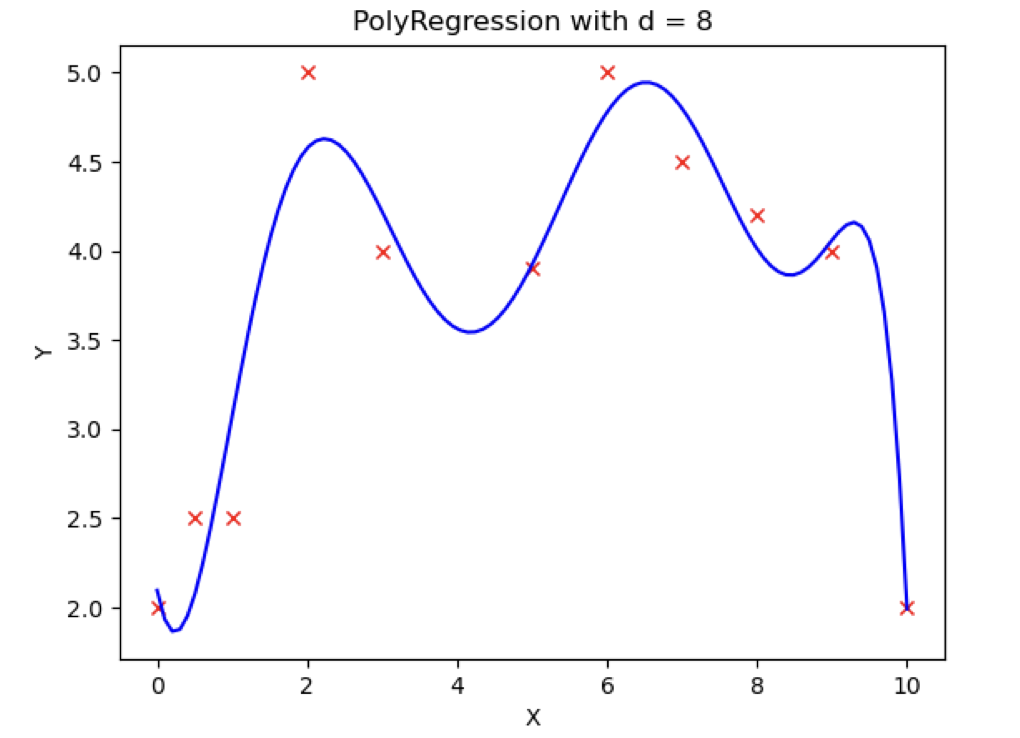
\includegraphics[width=0.4\textwidth]{../img/polyregDegree8.png}
        \vspace{-1em}
        \caption{Fit of polynomial regression with $\lambda = 0$ and $d = 8$}\label{fig:polyregUnivariate}
    \end{figure}

    By not including the $x_0$ column in the matrix \texttt{polyfeatures()}, this allows the \texttt{polyfeatures} function to be more general, so it could be applied to multi-variate data as well. (If it did add the $x_0$ feature, we'd end up with multiple columns of 1's for multivariate data.)\\
    
    Also, notice that the resulting features will be badly scaled if we use them in raw form.  For example, with a polynomial of degree $d = 8$ and $x = 20$, the basis expansion yields $x^1 = 20$ while $x^8 = 2.56 \times 10^{10}$ -- an
    absolutely huge difference in range.  Consequently, we will need to standardize the data before solving linear regression.  Standardize the data in \texttt{fit()} after you perform the polynomial feature expansion.  You'll need to apply the same standardization transformation in \texttt{predict()} before you apply it to new data.\\
    
    
    \item \points{2} Run \texttt{plot\_polyreg\_univariate.py} to test your implementation, which will plot the learned function.  In this case, the script fits a polynomial of degree $d=8$ with no regularization $\lambda = 0$.  From the plot, we see that the function fits the data well, but will not generalize well to new data points.  Try increasing the amount of regularization, and in 1-2 sentences, describe the resulting effect on the function (you may also provide an additional plot to support your analysis).
    
    
    \end{enumerate}
    
    \subsubsection*{What to Submit:}
    \begin{itemize}
        \item \textbf{Part a:} \textbf{Code} on Gradescope through coding submission.
        \item \textbf{Part b:} 1-2 sentence description of the effect of increasing regularization.
        \item \textbf{Part b:} Plots before and after increase in regularization.
        
    \end{itemize}
\end{aprob}

\newpage
\begin{aprob}
    \points{10} In this problem we will examine the bias-variance tradeoff through learning curves. Learning curves provide a valuable mechanism for evaluating the bias-variance tradeoff. 
    
        \item  Implement the \texttt{learningCurve()} function in \texttt{polyreg.py} to compute the learning curves for a given training/test set.  The \texttt{learningCurve(Xtrain, ytrain, Xtest, ytest, degree, regLambda)} function should take in the training data (\texttt{Xtrain}, \texttt{ytrain}), the testing data (\texttt{Xtest}, \texttt{ytest}), and values for the polynomial degree $d$ and regularization parameter $\lambda$. The function should return two arrays, \texttt{errorTrain} (the array of training errors) and \texttt{errorTest} (the array of testing errors).  The $i^{th}$ index (start from 0) of each array should return the training error (or testing error) for learning with $i +1$ training instances.  Note that the 0$^{th}$ index actually won't matter, since we typically start displaying the learning curves with two or more instances.\\
    
    When computing the learning curves, you should learn on \texttt{Xtrain}[0:$i$] for $i = 1, \ldots, \text{numInstances}(\texttt{Xtrain})$, each time computing the testing error over the {\bf entire} test set.  There is no need to shuffle the training data, or to average the error over multiple trials -- just produce the learning curves for the given training/testing sets with the instances in their given order.  Recall that the error for regression problems is given by
    \begin{equation}
        \frac{1}{n} \sum_{i=1}^n (h_{\bm{\theta}}(\mathbf{x}_i) - y_i)^2 \enspace.
    \end{equation}
    
    \item Once the function is written to compute the learning curves, run the \texttt{plot\_polyreg\_learningCurve.py} script to plot the learning curves for various values of $\lambda$ and $d$.  You should see plots similar to the following:
    \begin{figure}[ht!]
        \def\svgwidth{\textwidth}
        \centering
        \vspace{-1em}
        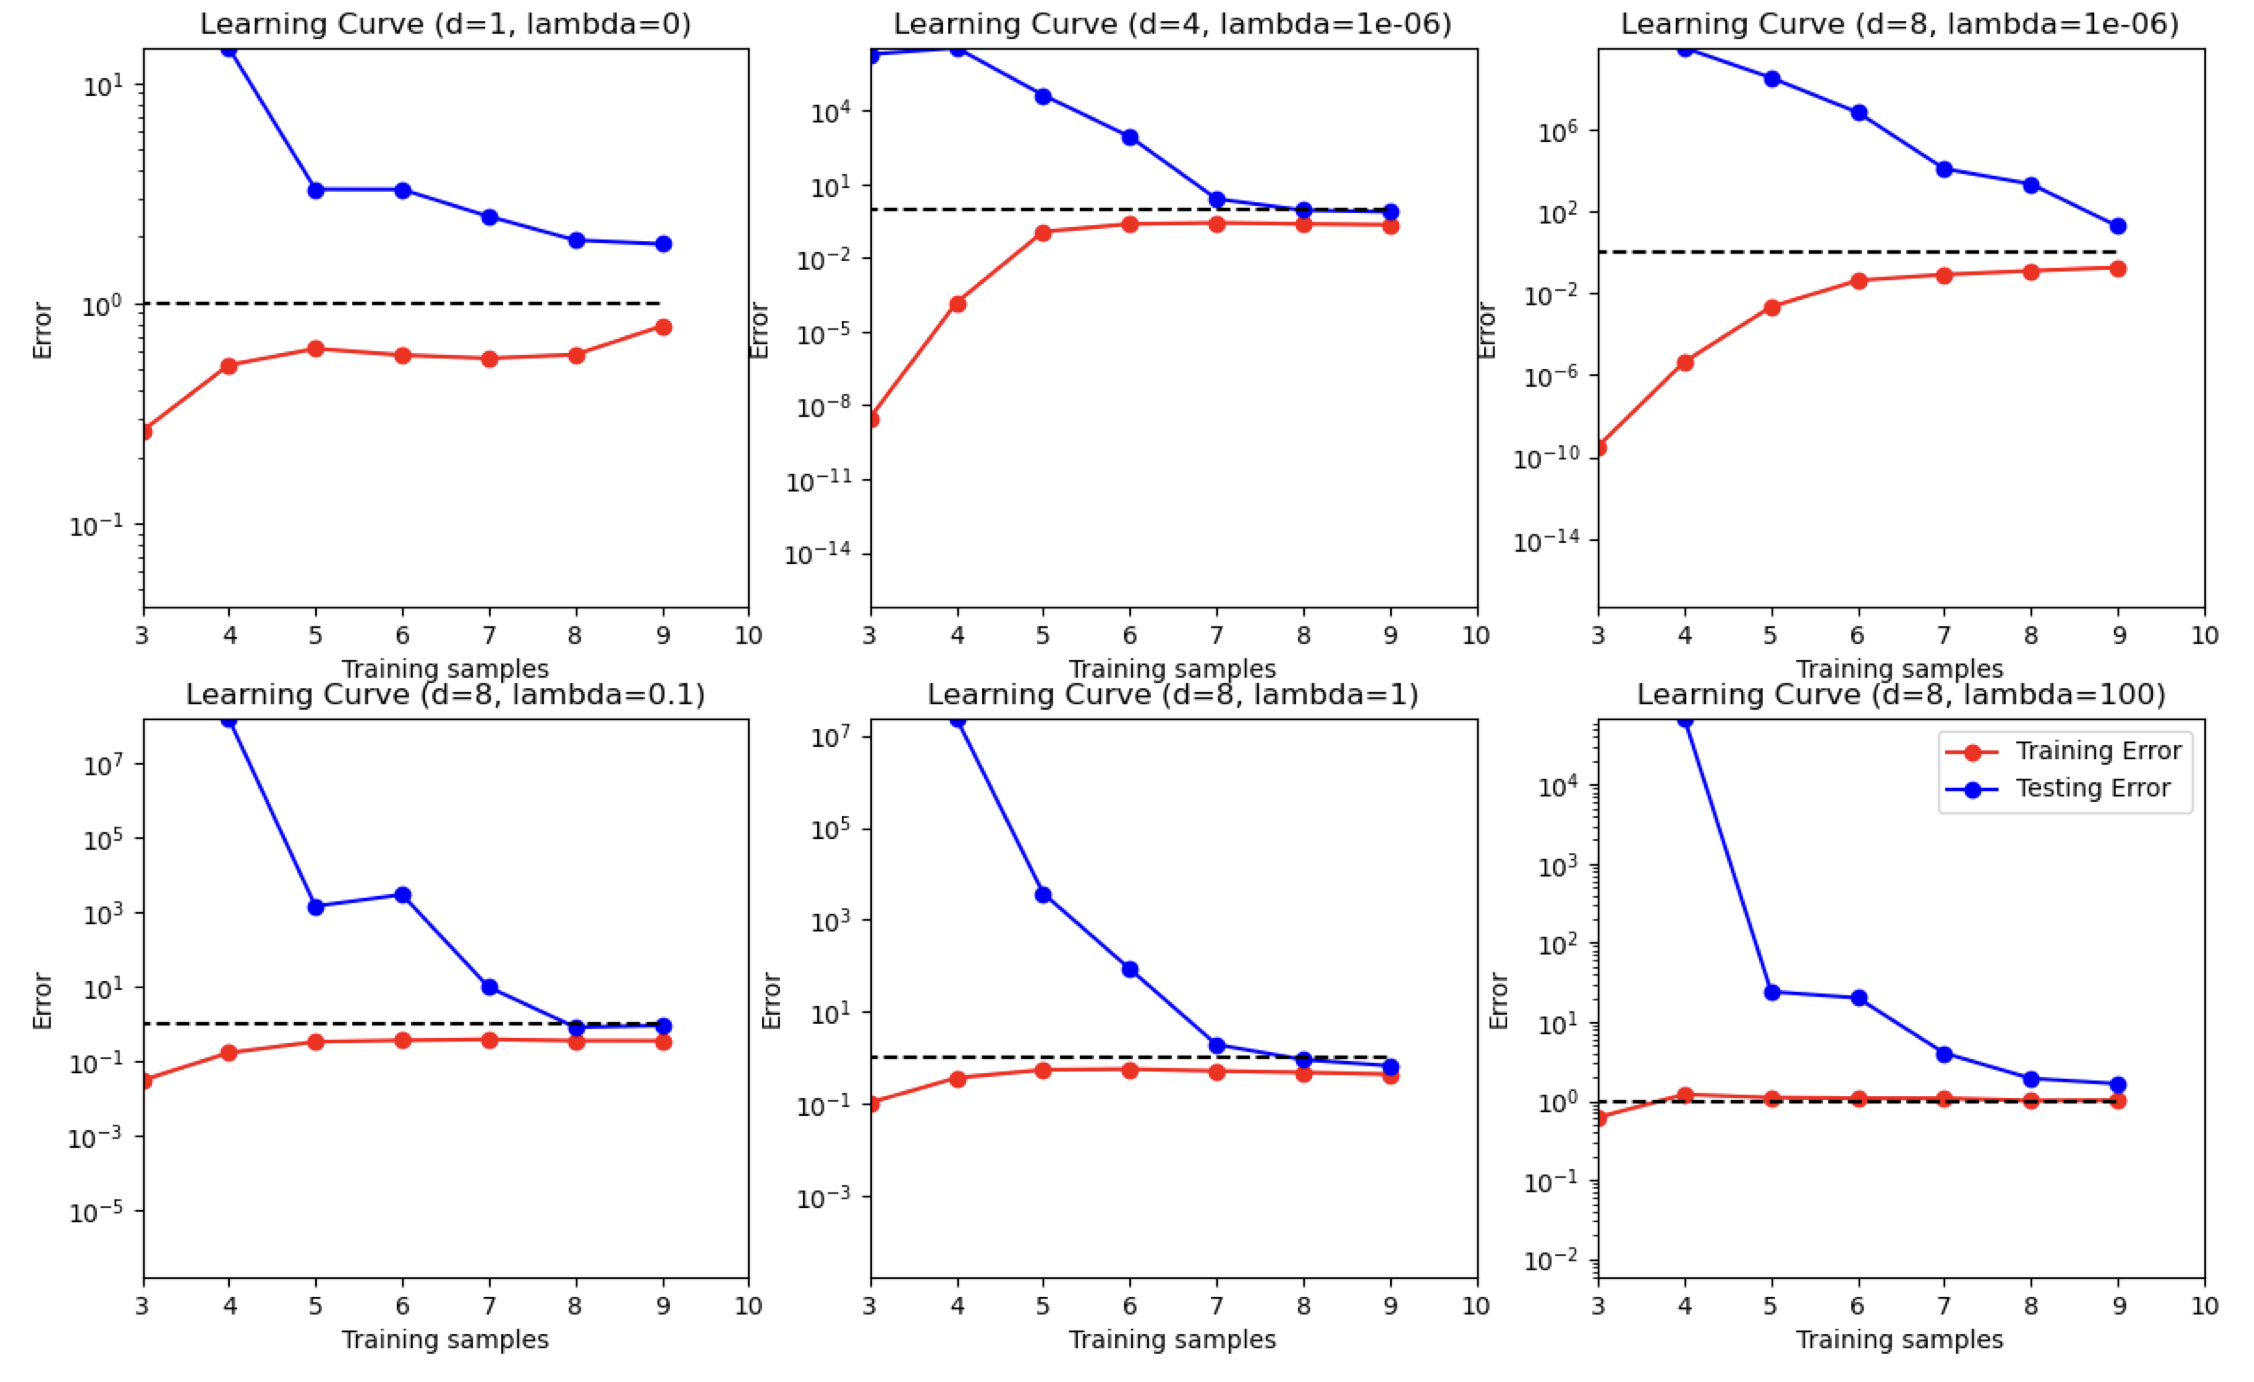
\includegraphics[width=\textwidth]{../img/polyregLearningCurves.png}
        \caption{Learning curves for various values of $d$ and $\lambda$. The blue lines represent the testing error, while the red lines the training error.}
    \end{figure}
    
    Notice the following:
    \begin{itemize}
        \item The y-axis is using a log-scale and the ranges of the y-scale are all different for the plots.  The dashed black line indicates the $y=1$ line as a point of reference between the plots.
        \item The plot of the unregularized model with $d = 1$ shows poor training error, indicating a high bias (i.e., it is a standard univariate linear regression fit).
        \item The plot of the (almost) unregularized model ($\lambda = 10^{-6}$) with $d = 8$ shows that the training error is low, but that the testing error is high.  There is a huge gap between the training and testing errors caused by the model overfitting the training data, indicating a high variance problem.
        \item As the regularization parameter increases (e.g., $\lambda = 1$) with $d = 8$, we see that the gap between the training and testing error narrows, with both the training and testing errors converging to a low value.  We can see that the model fits the data well and generalizes well, and therefore does not have either a high bias or a high variance problem.  Effectively, it has a good tradeoff between bias and variance.
        \item Once the regularization parameter is too high ($\lambda = 100$), we see that the training and testing errors are once again high, indicating a poor fit.  Effectively, there is too much regularization, resulting in high bias.
    \end{itemize}
    
    Submit plots for the same values of $d$ and $\lambda$ shown here. Make absolutely certain that you understand these observations, and how they relate to the learning curve plots.  In practice, we can choose the value for $\lambda$ via cross-validation to achieve the best bias-variance tradeoff.
    \\
    
    \textbf{Note: your learning curves slightly differ from ones above depending on whether you use `np.linalg.solve` or directly implement the closed-form solution. Both solutions are correct.}

    
    \subsubsection*{What to Submit:}
    \begin{itemize}
        \item \textbf{Plots} (or single plot with many subplots) of learning curves for $(d, \lambda) \in \{(1, 0), (4, 10^{-6}), (8, 10^{-6}), \\ (8, 0.1), (8, 1), (8, 100)\}$.
        \item \textbf{Code} on Gradescope through coding submission
    \end{itemize}
\end{aprob}

\clearpage{}

\section*{Ridge Regression on MNIST}
{\bf Relevant Files} (you should not need to modify any of the other files for this part):
\vspace{-1.2em}
\begin{multicols}{2}
    \begin{itemize}[noitemsep,nolistsep]
        \item \texttt{\bf ridge\_regression.py}
    \end{itemize}
\end{multicols}
\begin{aprob}
    In this problem, we will implement a regularized least squares classifier for the MNIST data set. The task
    is to classify handwritten images of numbers between $0$ to $9$.\\
    
    You are \textbf{NOT} allowed to use any of the pre-built  classifiers in \verb|sklearn|.  Feel free to use any method from \verb|numpy| or \verb|scipy|. {\bf Remember:} if you are inverting a matrix in your code, you are probably doing something wrong (Hint: look at \verb|scipy.linalg.solve|).\\

    \begin{figure}[h!]
        \centering
        \includegraphics[width=3in]{../img/mnist_images.png}
        \caption{Sample images from the MNIST data set.}
        \label{fig:mnist}
    \end{figure}

    Each example has features $x_i \in \R^d$ (with $d=28*28=784$) and label $z_j \in \{0,\dots,9\}$. \textbf{Since images are represented as 784-dimensional vectors, you can visualize a single example $x_i$ with \texttt{imshow} after reshaping it to its original $28 \times 28$ image shape} (and noting that the label $z_j$ is accurate). Checkout figure \ref{fig:mnist} for some sample images. We wish to learn a predictor $\widehat{f}$ that takes as input a vector in $\R^d$ and outputs an index in $\{0,\dots,9\}$. We define our training and testing classification error on a predictor $f$ as
    \begin{align*}
        \widehat{\epsilon}_{\textrm{train}}(f) &=
        \frac{1}{N _{\textrm{train}}} \sum_{(x,z)\in \textrm{Training Set}}     \1\{ f(x) \neq z \}
        \\
          \widehat{\epsilon}_{\textrm{test}}(f) &=
          \frac{1}{N _{\textrm{test}}} \sum_{(x,z)\in \textrm{Test Set}}     \1\{ f(x) \neq z \} 
    \end{align*}
    
    We will use one-hot encoding of the labels: for each observation $(x,z)$, the original label $z \in \{0, \ldots, 9\}$ is mapped to the standard basis vector $e_{z+1}$ where $e_i$ is a vector of size $k$ containing all zeros except for a $1$ in the $i^{\textrm{th}}$ position (positions in these vectors are indexed starting at one, hence the $z+1$ offset for the digit labels). We adopt the notation where we have $n$ data points in our training objective with features $x_i \in \R^d$ and label one-hot encoded as $y_i \in \{0,1\}^k$. Here, $k=10$ since there are 10 digits.
    
    \begin{enumerate}
        \item \points{10} In this problem we will choose a linear classifier to minimize the regularized least squares objective:
        \begin{align*}
            \widehat{W} = \text{argmin}_{W \in \R^{d \times k}} \sum_{i=1}^{n} \| W^Tx_{i} - y_{i} \|^{2}_{2} + \lambda \|W\|_{F}^{2}
        \end{align*}
        Note that $\|W\|_{F}$ corresponds to the Frobenius norm of $W$, i.e. $\|W\|_{F}^{2} = \sum_{i=1}^d \sum_{j=1}^k W_{i,j}^2$. To classify a point $x_i$ we will use the rule $\arg\max_{j=0,\dots,9} e_{j+1}^T \widehat{W}^T x_i$. Note that if $W = \begin{bmatrix} w_1 & \dots & w_k \end{bmatrix}$ then
        \begin{align*}
            \sum_{i=1}^{n} \| W^Tx_{i} - y_{i} \|^{2}_{2} + \lambda \|W\|_{F}^{2} &= \sum_{j=1}^k \left[  \sum_{i=1}^n ( e_j^T W^T x_i - e_j^T y_i)^2 + \lambda \| W e_j \|^2 \right] \\
            &= \sum_{j=1}^k \left[  \sum_{i=1}^n ( w_j^T x_i - e_j^T y_i)^2 + \lambda \| w_j \|^2 \right] \\
            &= \sum_{j=1}^k \left[  \| X w_j - Y e_j\|^2 + \lambda \| w_j \|^2 \right]
        \end{align*}
        where $X = \begin{bmatrix} x_1 & \dots & x_n \end{bmatrix}^\top \in \R^{n \times d}$ and $Y = \begin{bmatrix} y_1 & \dots & y_n \end{bmatrix}^\top \in \R^{n \times k}$. Show that
        \begin{align*}
            \widehat{W} = (X^T X + \lambda I)^{-1} X^T Y
        \end{align*} 

        \bigskip
        
        \item \points{9} 
        \begin{itemize}
            \item Implement a function \verb|train| that takes as input $X \in\R^{n \times d}$, $Y \in \{0,1\}^{n \times k}$, $\lambda > 0$ and returns $\widehat{W} \in \R^{d \times k}$.
            \item Implement a function \verb|one_hot| that takes as input $Y \in \{0, ..., k-1\}^{n}$, and returns $Y \in \{0,1\}^{n \times k}$.
            \item Implement a function  \verb|predict| that takes as input $W \in \R^{d \times k}$, $X' \in\R^{m \times d}$ and returns an $m$-length vector with the $i$th entry equal to $\arg\max_{j=0,\dots,9} e_j^T W^T x_i'$ where $x_i' \in \R^d$ is a column vector representing the $i$th example from $X'$.
            \item Using the functions you coded above, train a model to estimate $\widehat{W}$ on the MNIST training data with $\lambda = 10^{-4}$, and make label predictions on the test data. This behavior is implemented in the \verb|main| function provided in a zip file.
        \end{itemize}
        
         \item \points{1} What are the training and testing errors of the classifier trained as above?

        \item \points{2} Using matplotlib's \texttt{imshow} function, plot any 10 samples from the test data whose labels are incorrectly predicted by the classifier. Notice any patterns?
    \end{enumerate}
    Once you finish this problem question, you should have a powerful handwritten digit classifier! Curious to know how it compares to other models, including the almighty \textit{Neural Networks}? Check out the \textbf{linear classifier (1-layer NN)} on the {\color{blue}\href{http://yann.lecun.com/exdb/mnist/}{official MNIST leaderboard}}. (The model we just built is actually a 1-layer neural network: more on this soon!)
    \subsubsection*{What to Submit:}
    \begin{itemize}
        \item \textbf{Part a:} Derivation of expression for $\widehat{W}$
        \item \textbf{Part b:} \textbf{Code} on Gradescope through coding submission
        \item \textbf{Part c:} Values of training and testing errors
        \item \textbf{Part d:} Display of 10 images whose labels are incorrectly predicted by the classifier. 1-2 sentences reasoning why.
    \end{itemize}
\end{aprob}

\section*{Administrative}
\begin{aprob}
\begin{enumerate}
    \item \points{2} About how many hours did you spend on this homework? There is no right or wrong answer :)
\end{enumerate}
\end{aprob}

\end{document}
